\documentclass[noamssymb,svgnames]{beamer}
\usecolortheme{beaver}
\usefonttheme{serif}
\usefonttheme{professionalfonts}

\usepackage[bitstream-charter]{mathdesign} % Use BT Charter font
\usepackage{beramono}                      % Use Vera Mono for \ttfamily
\usepackage[T1]{fontenc}                   % Use T1 encoding instead of OT1
\usepackage[utf8]{inputenc}                % Use UTF8 input encoding
\usepackage{microtype}                     % Improve typography
\usepackage{booktabs}
\usepackage[binary-units]{siunitx}
\usepackage{tikz}
\usetikzlibrary{shapes.geometric}

\usepackage{hyperref}
\hypersetup{pdfstartview=Fit}

% BEAMER CONFIGURATION ---------------------------------------------------------
\setbeamerfont{block title}{size=\normalsize}
\setbeamerfont{block body}{size=\scriptsize}
\setbeamercolor{block title}{fg=darkred,bg=gray!10!white}
\setbeamercolor*{item}{fg=darkred}

% TCOLORBOX / MINTED CONFIGURATION ---------------------------------------------
\usepackage[many,minted]{tcolorbox}
\setminted{
  mathescape,
  autogobble,
  fontfamily=courier,
  framesep=2mm
}

% ------------------------------------------------------------------------------
\title{Working on Development}

\institute{
\includegraphics[width=2in]{../images/openmc_logo.png}}

\date{OpenMC Workshop \\ Canadian Nuclear Laboratories \\ March 14--16, 2017}

% ------------------------------------------------------------------------------
\begin{document}

\frame{\titlepage}

% ------------------------------------------------------------------------------

\begin{frame}{Fortran}
  \begin{itemize}
  \item Adhere to Fortran 2008 standard
  \item Extensive use of modules, derived types
  \item Uniform ``feel'' for code --- style guide
  \item Code is much more ``readable'' than other transport codes $\implies$
    easier learning curve
  \end{itemize}
\end{frame}

\begin{frame}{Python}
  \begin{itemize}
  \item Follow ``the'' Python style guide, PEP8
  \item All functions/classes must be documented
    \begin{itemize}
    \item ``docstrings'' are used to build HTML documentation
    \end{itemize}
  \item Compatible with Python 2.7 and 3.2+
  \item Limit use of non-standard library modules
  \end{itemize}
\end{frame}

\begin{frame}{Major modules --- Initialization}
  \begin{itemize}
  \item\textbf{initialize} --- Overall logic for initialization, reading
    command line arguments, starting up MPI, etc.
  \item\textbf{input\_xml} --- Read and parse data from input XML files.
  \item\textbf{xml\_interface} --- Functions for converting string data in XML
    to numbers, arrays, etc.
  \item\textbf{nuclide\_header} --- Logic for reading continuous-energy HDF5 data
  \item\textbf{tally\_initialize} --- Sets up data structures that allow for
    efficient tallying during the simulation.
  \end{itemize}
\end{frame}

\begin{frame}{Major modules --- Simulation}
  \begin{itemize}
  \item\textbf{geometry} --- distance to boundary, finding cells, point in
    cell, surface/lattice crossing, etc.
  \item\textbf{cross\_section} --- Calculate and store cross sections at
    specific energy/temperature
  \item\textbf{physics} --- Moving particle, sampling reaction, collision
    physics, sampling secondary angles/energies, fission site creation, etc.
  \item\textbf{tally} --- Score to tallies (collision/analog, track-length),
    accumulate scores at end of batch, calculate statistics
  \item\textbf{eigenvalue} --- Logic for $k$-eigenvalue calculation, fission
    bank syncronization, Shannon entropy, combined $k$ estimator
  \item\textbf{fixed\_source} --- Logic for fixed source calculation
  \end{itemize}
\end{frame}

\begin{frame}{Major modules --- End of simulation}
  \begin{itemize}
  \item\textbf{finalize} --- Overall logic for finishing run
  \item\textbf{state\_point} --- Create HDF5 state points that contain tally
    results, source sites, metadata, etc.
  \item\textbf{summary} --- Create geometry summary file
  \item\textbf{output} --- Write plain ASCII files and standard output
  \end{itemize}
\end{frame}

\begin{frame}{Other modules worth mentioning}
  \begin{itemize}
  \item\textbf{*\_header} --- ``Headers'' containing derived types
  \item\textbf{random\_lcg} --- Sampling pseudorandom numbers from linear
    congruential generator
  \item\textbf{plot} --- Create rasterized plots (PPM) that can easily be
    converted to PNGs
  \item\textbf{volume\_calc} --- Stochastic volume calculations
  \item\textbf{list\_header, set\_header, dict\_header, stl\_vector} --- Provide
    implementation of linked lists, sets, dictionaries, and vectors
  \item\textbf{pugixml/} --- C++ library for parsing XML
  \end{itemize}
\end{frame}

\begin{frame}{Development}
  \begin{itemize}
  \item Version control through \textbf{git}
  \item Code hosting, bug tracking through \textbf{github}
    \begin{itemize}
    \item\url{https://github.com/mit-crpg/openmc}
    \end{itemize}
  \item Automatic documentation generation with \textbf{Sphinx}
    \begin{itemize}
    \item\url{http://mit-crpg.github.com/openmc}
    \end{itemize}
  \end{itemize}
\end{frame}

\begin{frame}{Repository on Github}
  \begin{itemize}
  \item View/obtain source code
  \item Report bugs and issues
  \item Pull requests
  \item Online documentation
  \end{itemize}
\end{frame}

\begin{frame}{Continuous Integration}
  \begin{itemize}
  \item Regression test suite consisting of 82 problems
  \item Every time pull request is submitted/updated, Travis CI:
    \begin{itemize}
    \item Installs gcc, g++, cmake, etc.
    \item Installs Python and third-party packages
    \item Downloads HDF5 data
    \item Builds OpenMC
    \item Runs test suite on both Python 2.7 and Python 3.4, with several
      different build configurations
    \end{itemize}
  \end{itemize}
\end{frame}

\begin{frame}{Why you should use OpenMC}
  \begin{itemize}
  \item Free from licensing/export control issues
  \item State-of-the-art code that is intuitive, well-commented, with a
    relatively low learning curve. Time-to-meaningful-development is much less
    than MCNP or other codes!
  \item Version control (esp. branching and workflow) is extremely clean and
    smooth
  \item Collaboration with other organizations
  \item Opportunity to contribute back to the community
  \end{itemize}
\end{frame}

\begin{frame}{How to get started}
  \begin{enumerate}
  \item Create an account on GitHub
  \item Fork the code on GitHub
  \item Hack away!
  \item If you want to contribute back, issue a ``pull request''
  \end{enumerate}
\end{frame}

\begin{frame}{Guidelines for Review}
  \begin{itemize}
  \item Clear purpose and useful
  \item Compiles under all configurations, passes test suite
  \item Test cases are added, if appropriate
  \item Conforms to style guide
  \item New features/input documented
  \item No unnecessary software dependencies introduced
  \end{itemize}
\end{frame}

\begin{frame}{Integration manager workflow}
  \begin{center}
    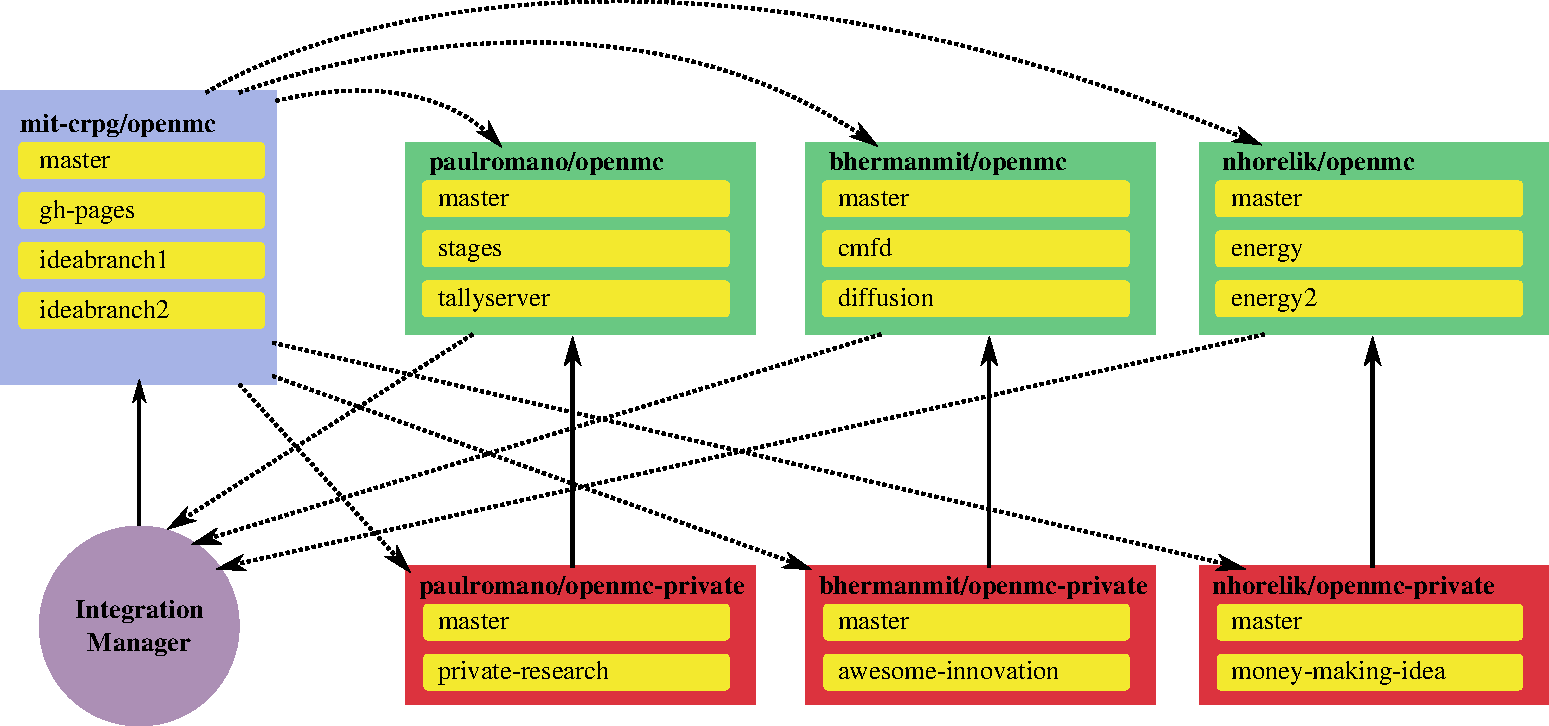
\includegraphics[width=\textwidth]{../images/integration-manager.pdf}
  \end{center}
\end{frame}

\begin{frame}{Rewrite in C++}
  Core developers agree a rewrite of the core codebase in C++ would be
  worthwhile:
  \begin{itemize}
  \item Use of external libraries written in C/C++
  \item Standard-library containers and algorithms
  \item Interoperating with other community codes: MOOSE, Shift, Geant, PyNE
  \item Structure as a library
  \item Developer talent pool
  \end{itemize}
\end{frame}

\begin{frame}{Contact}
  \begin{itemize}
  \item Work Email: promano@anl.gov
  \item Personal Email: paul.k.romano@gmail.com
  \item Work Tel.: +1 630 252-6779 (Wed-Fri)
  \end{itemize}
\end{frame}

\end{document}
